\section{Theory and experimental setup}

\subsection{General explanation about plasma}
Though every gas always has a small degree of ionisation, plasma has some defining qualities [which sets it apart][which require a separate description][which justify the need to properly define it [the need for a proper definition]].
[A common definition of plasma is that of a] [a simple textbook definition would be a] \emph{quasineutral} gas of charged and neutral particles which exhibits \emph{collective} behaviour \cite{chen_introduction_2006}.
[The concepts of quasineutrality and collectivity need further explanation.]
[While this may seem precise, we must define what quasineutral and collective means]

Quasineutrality is a mathematical way of saying that even though the particles making up a plasma consist of free electrons and ions, 
their overall charge densities cancel each other in equilibrium\cite{gibbon_introduction_2016}.
In other words, if $n_e$ and $n_i$ are respectively the number densities of electrons and ions with charge number $Z$, then these are locally balanced, i.e.
\begin{equation}
    n_e \simeq Z n_i
\end{equation}
This property is closely related to the phenomenon of Debye shielding:
if hypothetically we tried to put an electric field inside a plasma by inserting two spheres with charges of opposite sign and absolute value $Q$, almost immediately a cloud of ions would surround the negative sphere and a cloud of electrons the positive sphere, in such a way as to shield the newly created field.
The effectiveness of this shielding will depend on the electron temperature $T_e$, as the thermal agitation of the particles allows them to escape the electrostatic potential well.
Though ions and electrons often have separate Maxwellian distributions with different temperatures, it is the electron temperature which is considered because the ions are less mobile and rarely contribute to the shielding\cite{chen_introduction_2006}.
The potential $\phi(r)$ around the spheres after the readjustement of the charges has taken place can be calculated \cite{sanjines_notice_2014}:
\begin{equation}
    \phi(r) = \frac{Q}{4\pi \epsilon_0 r} e^{-r / \lambda_d} \quad \mathrm{with} \quad \lambda_d = \sqrt{\frac{\epsilon_0 K_B T_e}{n_0 e^2}}
\end{equation}
where $n_0 \simeq n_i$ is the gas number density\cite{gibbon_introduction_2016}.
The characteristic length $\lambda_d$ inside the exponential, known as \emph{Debye length}, is a measure of the shielding distance around the sphere.
As such, another criterion to define a plasma is for $\lambda_d$ to be much smaller than the size of the system.

The term collective behaviour refers instead to the fact that as the charged particles move around, they generate both local concentrations of positive or negative charges, giving rise to electric fields, and currents, and so magnetic fields\cite{chen_introduction_2006}.
These fields can then affect other charged particles far away\footnotemark, which means that plasmas show a \emph{simultaneous} response of many particles to an external stimulus\footnotemark.
This is [very different] from the behaviour of a neutral gas, in which particles interact only during collisions as a result of the short-range van der Waals force \cite{piel_plasma_2017}.
\footnotetext{On peut mettre ici une description de l'action des champs sur des volumes de plasma, Section 1.2 \cite{chen_introduction_2006}.}
\footnotetext{Alternatively, "macroscopic fields usually dominate over short-lived microscopic fluctuations".}

[A third criterion is: collisions of charged particles with neutral atoms should be infrequent.]

In this study[work] we will deal with a cold plasma, i.e. a gas where ions are not thermalised and electrons have a temperature such that $T_e >> T_i$, in reason of their lower mass\cite{bagnato_notice_2019}.

\subsection{Langmuir probes}
\paragraph{How they work}
Langmuir probes are a measurement device used to determine different properties of plasma, for example electron temperature and density, in a point of the chamber.
They are widely used in plasma physics because of their simple construction and versatility.
They consist of a plane electrode, often a small tantalum disk, which is inserted into the chamber and which is biased by an external voltage \cite{piel_plasma_2017}.
We can then measure the probe current, generated by the charges (both ions and electrons) that reach the surface.

\paragraph{The I-V characteristic curve}
This behaviour of the current is described in the $I$--$V$ characteristic curve of the probe, a measure of the probe current itself as a function of the applied potential.

The characteristic curve can be subdivided into three regimes. At high negative bias (region I), no electrons reach the probe and a constant ion saturation current is extracted from the plasma. 
At high positive bias (region III), a constant electron saturation current is found. 
In the intermediate region II, called the electron retardation regime, part of the electrons can overcome the energy barrier and reach the probe \cite{piel_plasma_2017}. 
Though the measured current is a sum of ion and electron current, is is the electron current which dominates since we're dealing with cold plasma \cite{sanjines_notice_2014}.
According to the Boltzmann factor[???], the electron current increases exponentially with the bias voltage:
\begin{equation}
    I_{probe}(V_{probe}) = I_{e,sat} \frac{e^{q(V_{probe} - V_{bias})}}{K_B T_e} \quad \mathrm{Maybe change notation, not clear enough.}
\end{equation}

Two points of physical significance:
\begin{itemize}
    \item The floating potential $\Phi_f$, i.e. the probe potential at which no net current flows in the probe circuit is the boundary between regions I and II.
    \item The plasma potential $\Phi_p$ is the potential inside the ambient plasma, at the boundary between regions II and III. The current corresponding to this point is the electron saturation current, given by
    \begin{equation}
        I_{es} = \frac{1}{4}e n_e v_{e,th} A_{probe}
    \end{equation}
\end{itemize}

\paragraph{What did we do?}
Linearising the expression of current in region II we have:
\begin{equation}
    \ln\left(\frac{I_e}{I_e,sat} \right) = \frac{e(V_{probe} - V_{bias})}{k_B T_e}
\end{equation} 
A linear regression in this region allows then to get the electron temperature.

To get the electron density, we must first find the plasma potential by linear regression, plotting the logarithm of the current and fitting the two regions, II and III.
The crossing point of the two fits yields the plasma potential.
Evaluating the current at this potential and rearranging the equation in the following way:
\begin{equation}
    n_e = \frac{4}{e v_e A_p} I_{e,sat} = \frac{1}{e A_p} \sqrt{\frac{2 \pi m_e}{k_B T_e}} I_{e,sat}
\end{equation}
we get the density.

Figure with the different regions.

[Amazing description in Section 7.6 of \cite{piel_plasma_2017}]

\subsection{Ion-acoustic waves}
Plasma goes boing boing.

It is possible to induce a longitudal oscillation of the ions and electrons in a plasma. These types of waves are called "ion acoustic waves". In the context of our experiment, the plasma is at a low pressure, meaning that the wave can only propagate through the Coulomb force between charged particles, because collisions are too rare.
For plasmas composed of only 1 type of ion, and considering that the wavelength of the induced wave is much larger than the Debye length $\lambda_d$, the ion-acoustic waves are disperionless, meaning $v_s = \omega/k = \lambda \nu$. The expression for the speed of the wave is then
\begin{equation}
    v_s eq
\end{equation}
M mass of ion, Z charge of ion, which in this experiment we set to $18$ because of Argon, $T_e$/$T_i$ electron/ion temp, and $\gamma_e=3$/$\gamma_i=1$. With the approximations, and taking into account that we're dealing with a cold plasma, we can simplify this expression to
\begin{equation}
    eq v_s simplified
\end{equation}
% this speed can be interpreted as the thermal speed the ions would have if they were at the electron's temperature
If we then measure the speed of the propagating wave we can find the electron temperature. We measured the speed by inducing an ion-acoustic wave at a specific frequency, and measuring the wavelength by moving the probe and measuring the position of the maxima of the wave.

\subsection{Experimental setup}
We have a chamber and two probes (one like this, the other like that) and a bunch of voltage sources.
Also two tungsten filaments to heat the whole thing up.
With two voltage sources attached.
Also the grill and the cage and the whole thing is grounded but not really.

And here a very nice figure with the schematics of the setup.
\begin{figure}
    \centering
    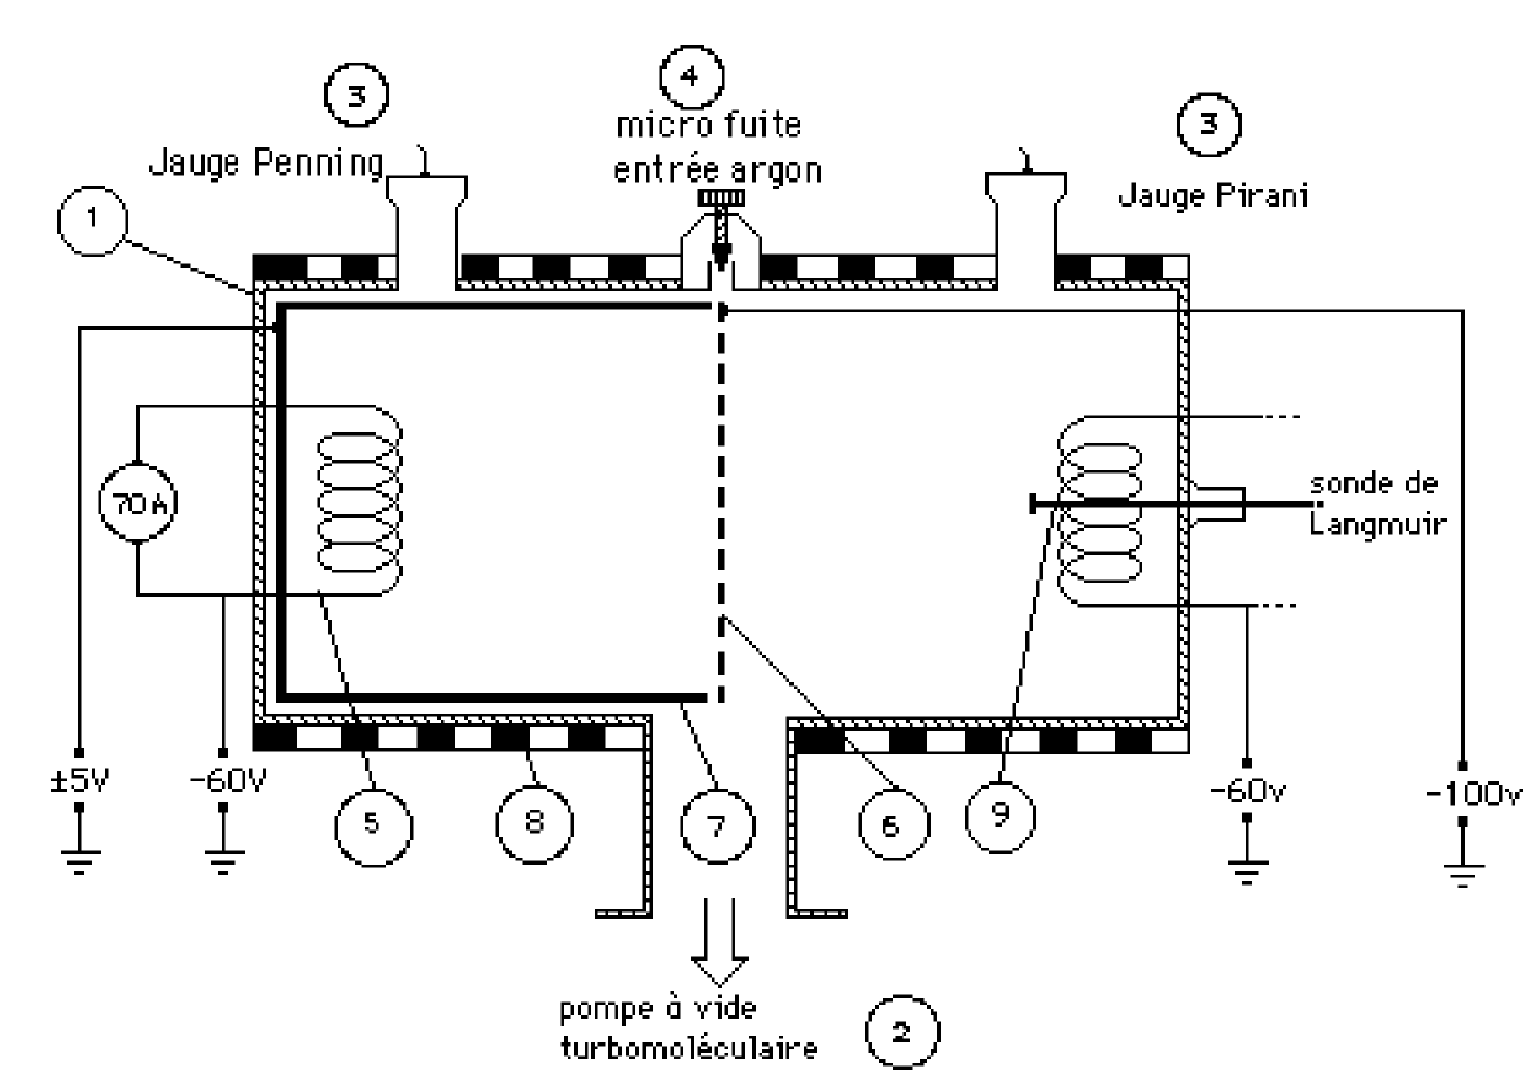
\includegraphics[width=12cm]{figures/experimental-setup.png}
    \caption{The experimental setup}
    \label{fig:experimental_setup}
\end{figure}

The plasma is produced by electron impact ionization
of argon atoms by electrons that are thermionically emitted and accelerated
from a hot tungsten filament.

\cite{merlino_understanding_2007} a une explication magnifique de à quoi est-ce que ça sert les aimants.
Aussi il explique bien la courbe I-V, si on a besoin de citer quelque chose on peut balancer ça.